\documentclass[en]{../../../../../../eplexam}

\usepackage{todonotes}
\usepackage{listings}
\usepackage{csquotes}
\usepackage{booktabs}
\usepackage{placeins}
\graphicspath{{img/}}

\newcommand{\proitem}{\item[\textbf{\color{green!80!black}{$+$}}]}
\newcommand{\consitem}{\item[\textbf{\color{red!80!black}{$-$}}]}

\hypertitle{Programming paradigms}{8}{SINF}{2335}{2016}{Juin}{All}
{Florian Thuin}
{Sebastian Gonzales}

\section{Define the following concepts in your own words, and give
a concrete example or counterexample for each of them,
taken from your own experience.}

\begin{description}
    \item[reification]: making the language concepts available for manipulation by the programmer.
        \subitem Example: in Ruby, the class \verb#Class# represents a class.
        \subitem Example: the \lstinline[language=java]|java.lang.Class| $\rightarrow$ \lstinline[language=java]|newInstance()|,
        getConstructors(),\ldots
    \item[metaprogramming]: ability of a program to reason about another. A metaprogram is a program whose data corresponds to another program. It can be a different program, or itself.
        \subitem Examples : PyLint, JVM, gdb, checkstyle.
    \item[reflection]: ability of a program to examine or change its own implementation at runtime. A reflexive program is a program whose data corresponds to itself.
        \subitem Example : Machine-Learning programs, testing frameworks
        (ScalaTest?).
    \item[introspection]: ability of a program to examine its own state.
        \subitem Example : inspecting the details of a class (Ruby: 
        \verb#my_obj.instance_of?(Object)#)
    \item[intercession]: ability of a program to change its behaviour.
        \subitem Example : adding/removing a method to a class (Ruby: 
        \verb#remove_method#)
    \item[structural reflection]: ability to change aspects (properties) of a
    program.
        \subitem Example : adding instance variables.
    \item[behavioural reflection]: ability to modify the behaviour of a program at runtime.
        \subitem Example : modify method dispatching mechanism.
    \item[meta-object protocol]: architecture defining how the components of the system interact.
        \begin{figure}[!ht]
            \centering
            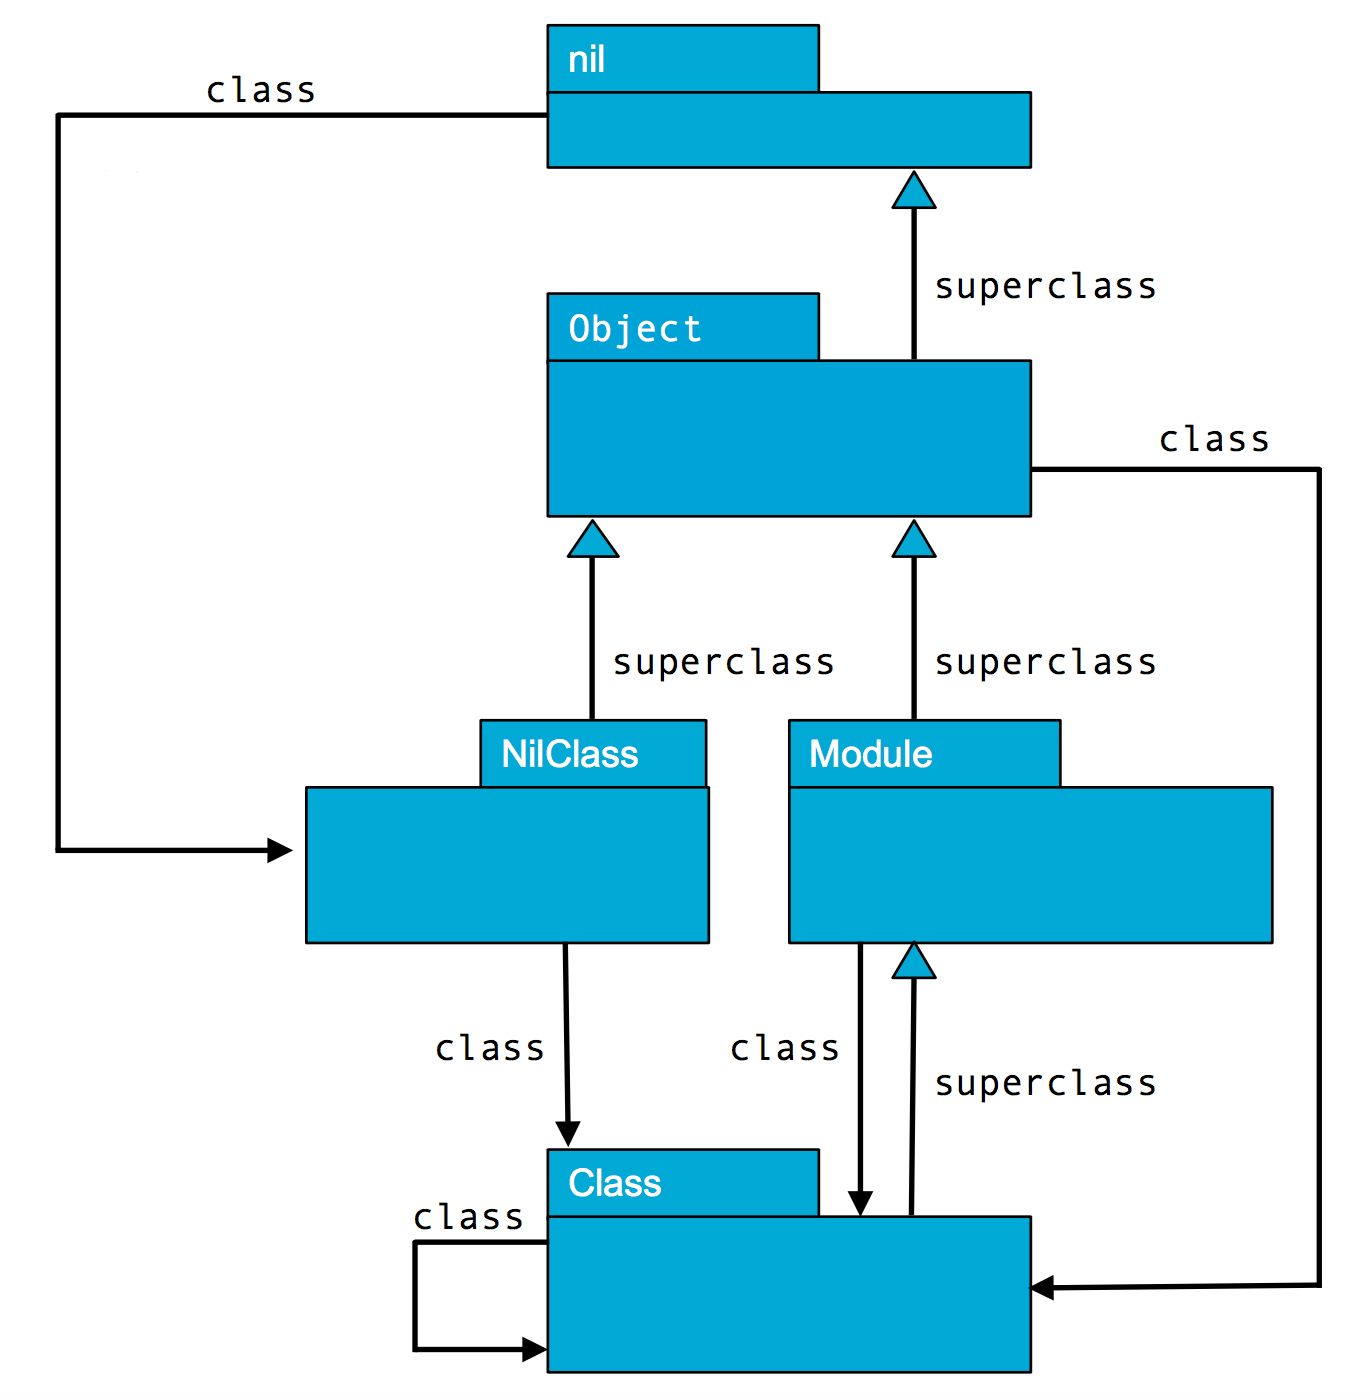
\includegraphics[width=0.5\linewidth]{mop_ruby.png}
            \caption{Example: Ruby's MOP}
        \end{figure}
        \FloatBarrier

        \begin{figure}[!ht]
            \centering
            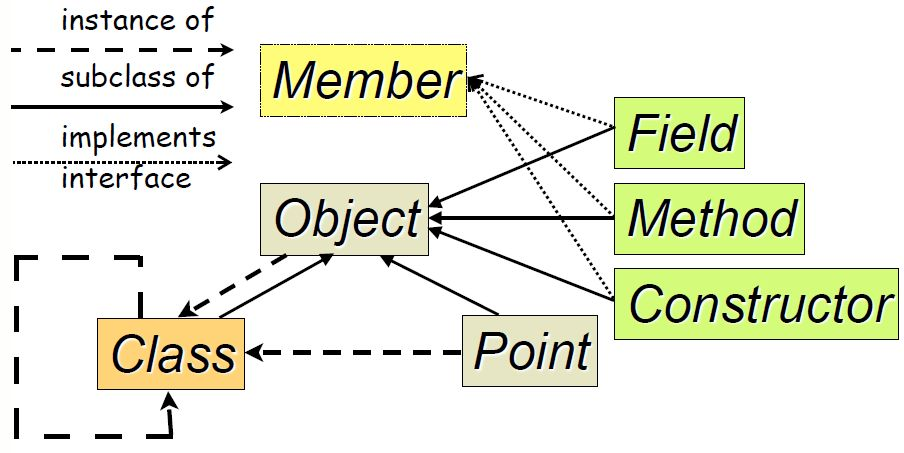
\includegraphics[width=0.6\linewidth]{mop_java.png}
        \end{figure}
    \item[macros]: A macro is an identifier which will be replaced by a piece of code during the compilation. An example is the \verb$#define$ in C.
    Starting with \verb$#define TEST 100$, and later in the code \verb#i = TEST 2;# will lead to replace TEST by 100 during the compilation (and thus $i = 100 - 2;$) \newline

    Class-level methods that generate code behind the scenes. We can also define our own macros.
        \subitem Example : In Ruby, definition of accessors. Here, generate the accessors.

        \begin{lstlisting}
attr_reader :x, :y
attr_writer :x, :y
        \end{lstlisting}
    \item[bootstrapping]: is the use of a trick, a special process in order to perform a task that is generally impossible. For instance, we can build a very complex program nearly impossible to create from scratch just
    by bootstrapping it with few basic programs.
        \subitem Example : writing a compiler in terms of itself. (see question 7 for a real example)
    \item[metaclass]: describes the class behaviour and state (subclasses,
    method dictionary, etc).
        \subitem Example: in SmallTalk, the class \verb#SmallInteger# has a meta
        class \verb#SmallInteger class# in which, among others, we can find the
        class methods.
\end{description}

\section{Explain the difference between introspection and
intercession. Illustrate with concrete examples taken from
the course or from another language which you have
studied.}

\begin{description}
    \item[Introspection]: ability of a program to examine its own state.
        \subitem Example : inspecting the details of a class (Ruby: 
        \verb#my_obj.instance_of?(Object)#)
    \item[Intercession]: ability of a program to change its behaviour.
        \subitem Example : adding a method to a class (Ruby:
        \verb#remove_method#)
\end{description}
\section{Explain the difference between structural and behavioural
reflection. Illustrate with concrete examples taken from the
course or from another language which you have studied.}

\begin{description}
    \item[Structural reflection]: ability to change aspects (properties) of a
        program.
        \subitem Example : adding instance variables.
    \item[Behavioural reflection]: ability to modify the behaviour of a program
        at runtime.
        \subitem Example : modify method dispatching mechanism.
\end{description}


\section{Explain the difference between metaprogramming and
reflection. Illustrate with concrete examples taken from the
course or from another language which you have studied.}

\begin{description}
    \item[Metaprogramming]: program whose data corresponds to another program .
    It can be a different program, or itself.
        \subitem Examples : PyLint, JVM, gdb.

        \begin{figure}[!ht]
            \centering
            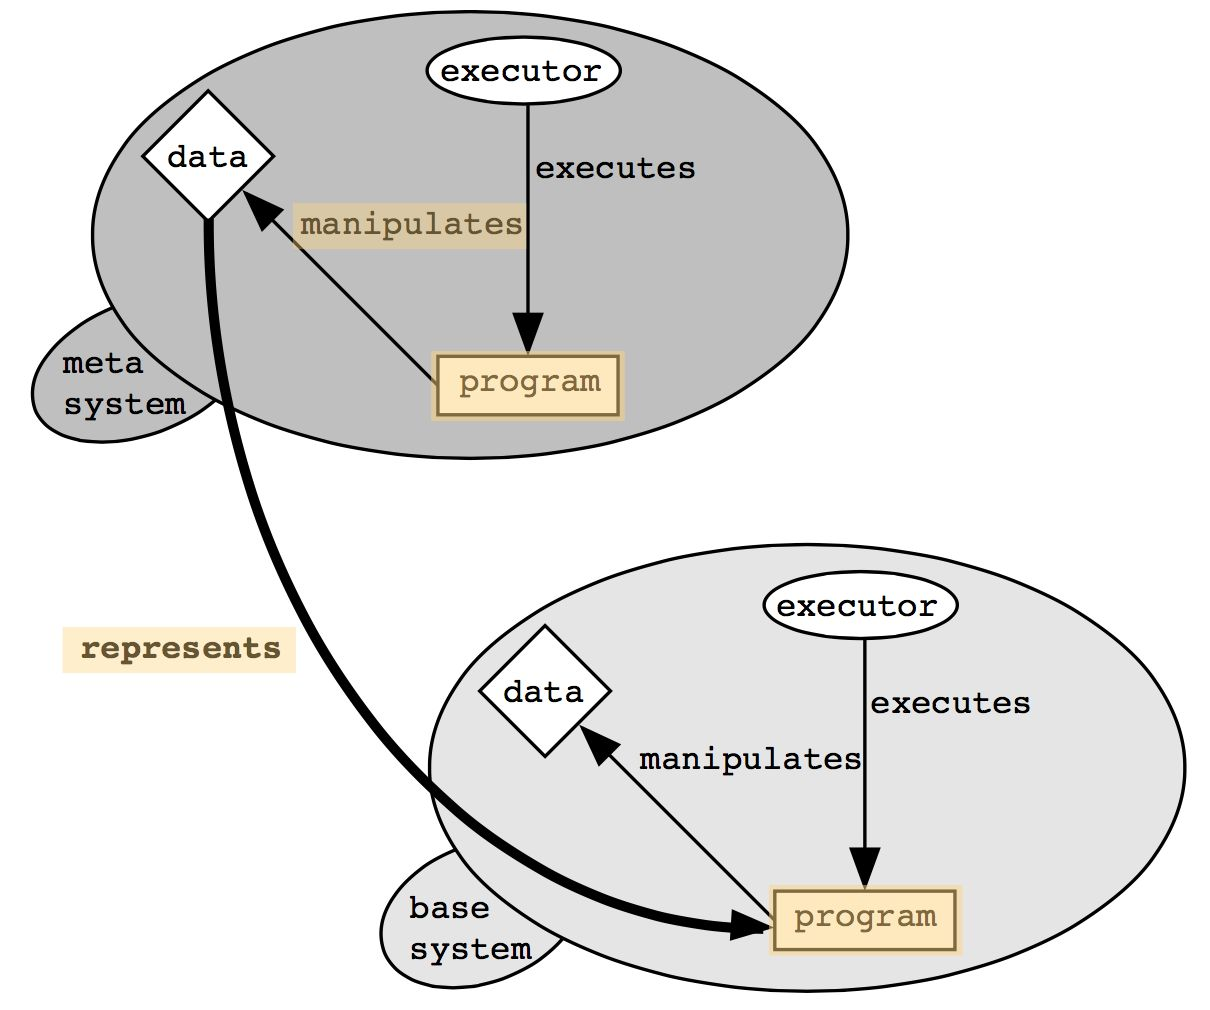
\includegraphics[width=0.5\linewidth]{meta_programming.png}
        \end{figure}
        \FloatBarrier

    \item[Reflection]: program whose data corresponds to itself.
        \subitem Example : Machine-Learning programs, testing frameworks
        (ScalaTest ?). For explanations about causal connection, see question
        8 ;-)

        \begin{figure}[!ht]
            \centering
            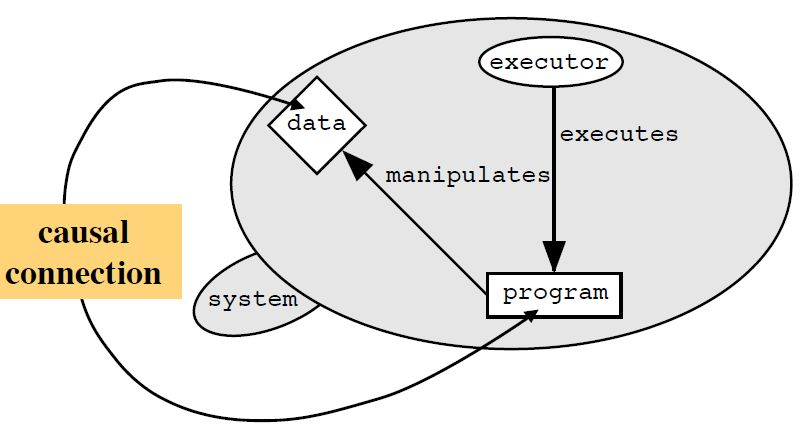
\includegraphics[width=0.5\linewidth]{reflection.png}
        \end{figure}
        \FloatBarrier
\end{description}


\section{What kinds of reflection can be distinguished? (Based on what is
reflected as well as based on when reflection takes place.) Give a concrete
example of each of these kinds of reflection, taken from your own experience or
assignments or from the theory course.}

\begin{description}
    \item[reflection]: program whose data corresponds to itself.
        \subitem Example: Machine-Learning programs, testing frameworks
        (ScalaTest ?).
    \item[introspection]: ability of a program to examine its own state.
        \subitem Example: inspecting the details of a class (Ruby: 
        \verb#my_obj.instance_of?(Object)#)
    \item[intercession]: ability of a program to change its behaviour.
        \subitem Example: adding a method to a class (Ruby:
        \verb#remove_method#)
    \item[structural reflection]: ability to change aspects (properties) of a
    program.
        \subitem Example : adding instance variables.
    \item[behavioural reflection]: ability to modify the behaviour of a
    program at runtime.
        \subitem Example : modify method dispatching mechanism.
    \item[compilation reflection]: ability to modify the program at compilation
    time.
        \subitem Example : macros.
    \item[runtime reflection]: ability to modify the program at runtime.
        \subitem Example : debugger.
\end{description}

\section{How do macros relate to reflection?
Do they provide a kind of reflection? What kind?}

Macros are identifiers that are replaced by a piece of code during the
compilation time. It is reflection because the program has a part that will be
changed at the compilation time, it’s then compilation reflection. One example
is the \verb$#define identifier text$ in C. Another example is the macro
\verb#attr_accessor :x# in Ruby which will generate getter and setter for the
attribute $x$ at compilation time.

\section{Can you give a concrete example of bootstrapping?
(If possible, taken from your own experience.)}

You want to do a Quine program in C. (A Quine program is a program that doesn’t
take any input, isn’t empty and outputs only its source code).\newline
The program has a code part and a data part where the data part represents the
entire code. The problem is that the data part is also contained in the code. We
need a trick in order to succeed : a bootstrap.\newline
This will consist to place a special character in the data part ( for example
\verb#@@@@#) and replace this special character by the data part when it will
be printed (only once). However, this isn’t metaprogramming (and thus no
reflection either) because the program doesn’t take as input a program.

\section{When defining reflection, we talked about \enquote{causal connection}.
What does this mean? What needs to be causally connected to what? Can you give
a concrete example? (If possible, taken from your own experience.) What happens
if you don’t have such a causal connection? Can we still speak about reflection
then? What kind?}

When two elements are causally connected, it means that if one of the two
changes, this will lead to an effect on the other. We have the same principle
in reflection between the program and the data he manipulates (where the data
is also the program). If we don’t have the causal connection, it’s not fully
reflective but we can still talk about reflection of the kind introspection (a
type of reflection where the program can inspect but not change itself).

Example (from course): robot arm

\begin{itemize}
    \item Domain: numbers indicating position of the arm.
    \item Updating coordinates: robot arm moves.
    \item Moving the robot arm: updates coordinates.
\end{itemize}

\section{Can you explain what the technique of scaffolding is? Can you give a
concrete example of scaffolding? We saw how to do scaffolding in Smalltalk.
How would you do it in language Y? Can you? What kind of reflection is needed
for that?}

A technique of scaffolding consists in a programming idiom that supports the
rapid development of prototypes.\newline

We can do scaffolding in the case we want a class that keeps some items in a
collection and that allows to enumerate over these elements by using
enumerators similar to those defined on the collection classes (by delegating
to the appropriate enumeration method defined on the collection). We can do
this in several ways.

\begin{itemize}
    \item We could implement manually all the item enumeration methods.
        \subitem[$\Rightarrow$]repetitive and not reflective.
    \item We could generate statically the methods because they have the same
    pattern (string replacement). In a concrete way, we start from one template
    of the methods and we build them and replace to correspond to the method
    we need.
        \subitem[$\Rightarrow$] Reflective but we have to set up at runtime the
        call to create all of these methods.
    \item We could also do dynamic forwarding thanks to the
    \verb#doesNotUnderstand# method. Every messages will be forwarded to the
    right collection method.
        \subitem[$\Rightarrow$] Reflective, similar to proxy.
    \item We could finally do a mix between the 2 and 3 where we use the
    \verb#doesNotUnderstand# to trigger the creation of the unknown methods
    (which will be created starting from the template defined in the second
    solution).
\end{itemize}

The kind of reflection that is needed is runtime reflection.\newline

In Ruby, the 4 methods are possible because there is also a mechanism similar
to the \verb#doesNotUnderstand# which is \verb#method_missing#. We could also
use the each method to iterate over the item and include the \verb#Enumerable#
mixin which will do the rest.\newline

In Java there isn’t such a method because of the static typing and we cannot
add dynamically a method at runtime (except with the trick of using the Java
Instrumentation to modify the bytecode which isn’t very clean), thus only the
first one is possible.

\section{What kinds of reflection do you need to implement a debugger like the
one provided by Smalltalk? Do the reflective features of language Y suffice to
build a similar debugger for that language? What kind of reflection is needed
for that?}

In Smalltalk, the debugger does intercession and introspection at runtime based
on the essential \verb#thisContext# which is the current stack. This stack is
just an object that we can modify. The type needed is then runtime reflection.
In Java it’s not possible to have a debugger as powerful because the
intercession is very limited. In Ruby it’s possible because there are plenty of
intercession features, similar to SmallTalk. Both Java and Ruby have the stack
as a copy and thus can just inspect it but not modify it on the fly like
SmallTalk does.

\section{Can you explain the Proxy design pattern and how reflection in
language Y could help to implement dynamic proxies? What kind of reflection is
needed for that?}

The proxy design pattern allows to provide a surrogate for another object in
order to control the access to it. The proxy keeps track of the object to which
it forwards requests. The proxy has an identical interface to clients. \newline
His use is then to serve as substitute when we don’t want (for security or
inconvenience (such as delay for expensive operation)) that the subject is
accessed directly.

\begin{figure}[!ht]
    \centering
    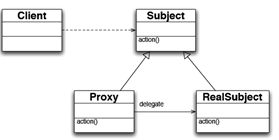
\includegraphics[width=0.5\linewidth]{proxy.png}
\end{figure}
\FloatBarrier

\paragraph{In Smalltalk\\}

The reflection in Smalltalk allows to implement dynamic proxies. \newline
We use Object Wrappers which consist of wrapping an object, capture all
messages that are sent to him and then handle or forward them. First we need to
create the Wrapper class. It will have a list of the selectors that the real
subject know and thanks to the dynamic typing, he will also have a reference to
this real subject. Two methods are necessary: the \verb#:wrap object# (wrap an
object) and \verb#doesNotUnderstand# (delegate the message to the real object
when in the selectors list). But we have a problem, when wrapping an object,
not all the references to the wrapped object are wrapped. In the wrap method,
we have to use the \verb#become# in order to switch all the references to the
wrapper. We have used some introspection such as retrieve all the selector of
the real object but we also used some intercession such as with \verb#become#
and \verb#doesNotUnderstand#.

\paragraph{In Ruby:\\}

Exactement la même chose qu’en Smalltalk, le \verb#doesNotUnderstand# à la Ruby
est \verb#missing_methods#. Par contre je sais pas s’il y a un équivalent du
\verb#become# de SmallTalk dans le but de faire en sorte que toutes les
références de l’objet wrappé pointent vers le wrapper (dans le cas ou on aurait
fait une référencé AVANT de wrapper).

\paragraph{In Java\\}
Depuis Java 1.3.
Principe : mm qu’en smalltalk. 

\todo[inline]{Pas trop, t'as pas d’équivalent de doesNotUnderstand ou de
\textit{method\_missing}, du coup tu dois avoir une interface avec toutes les méthodes
possibles pour l’objet réel, tu peux pas juste redéléguer. Ce role est rempli
par le Proxy qui va choper toutes les requêtes envoyées vers lui et vont être
déléguées vers le  InvocationHandler qui va choisir comment les traiter
(actions spécifiques plus invoke sur le réel objet qui est retenu dans le
invocationHandler) Par contre, tout comme le ruby, faut voir si y a pas
besoin du \textit{become} comme en SmallTalk pour que toute les références qui ont été
faites avant le proxy vers l’objet réel vont maintenant bien sur le proxy.}
Passer par un Proxy (class) et un invocationHandler (interface)

\section{What is the granularity of reflection in language Y? (What entities
are reified and what details of those entities are reified?) How does this
compare to language Z?}

Smalltalk and Ruby have both fully reflective languages. You can do intercession
and introspection. The entities are reified and there is a clear separation
between the meta and the base level.\newline
In Java, you can only do introspection and there isn’t a clear separation
between the meta and base level. However, you can also do some intercession
with the Java Instrumentation trick which consists to use agent in order to
modify bytecode (for example, it’s possible to replacing a class by another).
This is not clean and furthermore, you have to explicitly give an agent when
you launch the JVM, which isn’t very convenient.

\section{Concepts like reflection can be very powerful, but also
very dangerous if not used well.
In your opinion, when should / shouldn’t reflection be used?
Try to be as concrete as possible in your answer by giving
concrete examples from your own experience.}

\begin{itemize}
    \proitem Solution d’implémentation plus propre.
        \subitem Ex : comment appeler la méthode \verb#setColor# connue par les
        divers components graphiques dans des codes différents (achetés, fait
        par nous) ? Afin d’éviter les cast, les \verb#if#s,\ldots Peut se faire
        en 3 lignes de codes en Java + la gestion d’exceptions.
    \proitem Solution dynamique.
        \subitem Ex: récupérer de n’importe quel objet l’ensemble des variables
        d’instances de type int. Utiliser l’introspection au lieu d’implémenter
        dans chaque classe une méthode \verb#getIntVar()#.\newline

        Autre ex : programme qui permet à des gens novices dans la programmation
        de faire son propre programme (assez simple) avec des classes contenant
        des attributs et des méthodes.
    \consitem D’un point de vue sécurité, on peut modifier des variables
    d’instance.
        \subitem Ex: modifier l’amount de son compte.
    \consitem On peut modifier le \enquote{code source}.
        \subitem Ex: modifier le code de \verb#Fixnum# en Ruby et faire que le 
        $+$ (arithmétique) affiche \enquote{$1$} chaque seconde. Exemple un peu
        benêt, mais déjà bien ennuyant. Et on peut faire bien pire !
    \consitem Transformer le $+$ en $-$:
    \verb#class Fixnum; def + v; self ­ v; end; end#
\end{itemize}

\section{In the course introduction we talked about the Safir-Whorf hypothesis,
which said that (the choice of a particular) language may influence how one
sees and thinks about the world. Of course, this is only a hypothesis.
What is your opinion on this (in the context of programming languages).}

COP : \enquote{paradigm} $\rightarrow$ principe d’un programme qui s’adapte à des
critères divers en fonction du type de personne, de la position géographique,
de la situation,\ldots Il peut tant s’appliquer du côté UI, que du côté DB
voire même du côté business.

\bigskip
\begin{tabular}{lcc}
    \toprule
    & \textbf{Smalltalk} & \textbf{Java} \\
    \toprule
    \textbf{Syntax} & Simple & Complex \\
    \midrule
    \textbf{Typing} & Dynamic & Static (primitive types, type casts) \\
    \midrule
    \textbf{Reflection} & Full reflection & Introspection and some intercession \\
    \midrule
    \textbf{Garbage collection} & Yes & Yes \\
    \midrule
    \textbf{Virtual machine} & Yes & Yes \\
    \midrule
    \textbf{Concurrency} & Processes & Threads \\
    \midrule
    \textbf{Visibility of variables} & Protected & Public, protected, private \\
    \midrule
    \textbf{Visibility of methods} & Public & Public, protected, private \\
    \midrule
    \textbf{Dynamicity of methods} & Dynamic & Dynamic or static \\
    \midrule
    \textbf{Interfaces} & No & Yes \\
    \bottomrule
\end{tabular}

\end{document}
